\documentclass{article}
\usepackage[utf8]{inputenc}
\usepackage{graphicx}
\graphicspath{ {./images/} }
\usepackage{amsmath}
\usepackage{hyperref}
%\usepackage[english]{babel}

\usepackage[left=2cm,right=1cm, top=2cm,bottom=2cm,bindingoffset=0cm]{geometry}

\renewcommand{\normalsize}{\fontsize{14}{18pt}\selectfont}

\title{ Analyzis of E.coli strains for outbreak investigation via identification pathogenic genes    }
\author{ Kamilla Faizullina}
\date{\empty}

\begin{document}
\maketitle
\section{Introduction}
\section{Methods}
To analyze the E. coli X strains, I use the dataset from the TY2482 sample \cite{data}. To estimate genome size, I use Jellyfish \cite{jellyfish}. For estimation the genome size, the following formulas is used: 
$$ N = \frac{M*L}{L-K+1}, Genome\_size = \frac{N}{T}, $$
where N --- Depth of coverage, M --- k-mer peak, K --- k-mer-size, L --- average read length, T --- Total bases).

For assembling the genome the SPAdes tool is used \cite {spades}.

 


\section{Results}
I use Fastqc for \cite{fc} for estimation number of reads and quality control. Table 1 represents the number of reads of the sequencing data.  
I run Jellyfish tool only on the data labeled SRR292678. The length of mer is equal to 31. From the Figure 1, the peak position is $\approx 54$. $Genome\_size \approx 5 Gb$. %$ T = 549934690*90, N  \approx 98, Genome\_size \approx 5 Gb $.  
	\begin{table} 
	\centering
	\begin{tabular}{|c|c|c|}
		\hline
		The sequence & Reads \\
		\hline
		SRR292678 forward  &  5499346  \\
		\hline
		SRR292678 reverse &  5499346 \\
		\hline
		SRR292862 forward &  5102041 \\
		\hline
		SRR292862 reverse &  5102041 \\
		\hline
		SRR292770 forward  &  5102041 \\
		\hline
		SRR292770 reverse &   5102041  \\
		\hline
	\end{tabular}
	\caption{  Number of reads }
\end{table}


\begin{figure}[h]
	\centering
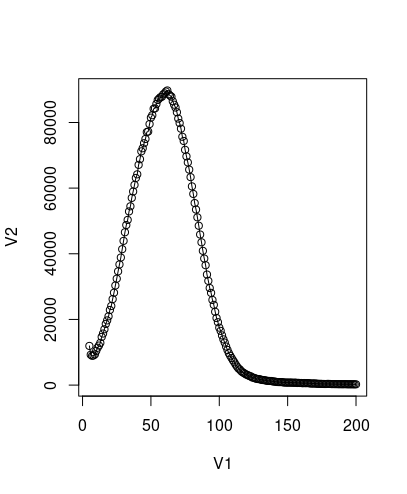
\includegraphics[scale=0.5 ]{peak1} 
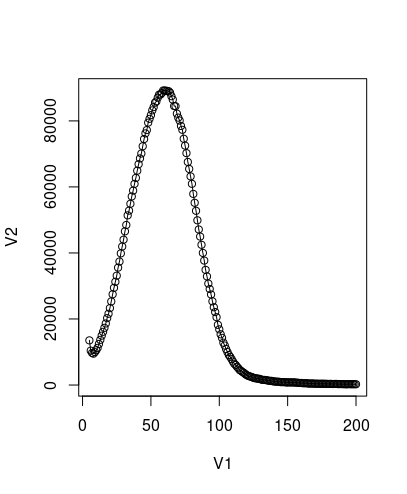
\includegraphics[scale=0.5 ]{peak2} \\
 
\centering \caption{The k-mer distribution in the forward and reverse data among region between 8 and 200}
\label{saw}
\end{figure}
 
\begin{figure}[h]
	\centering
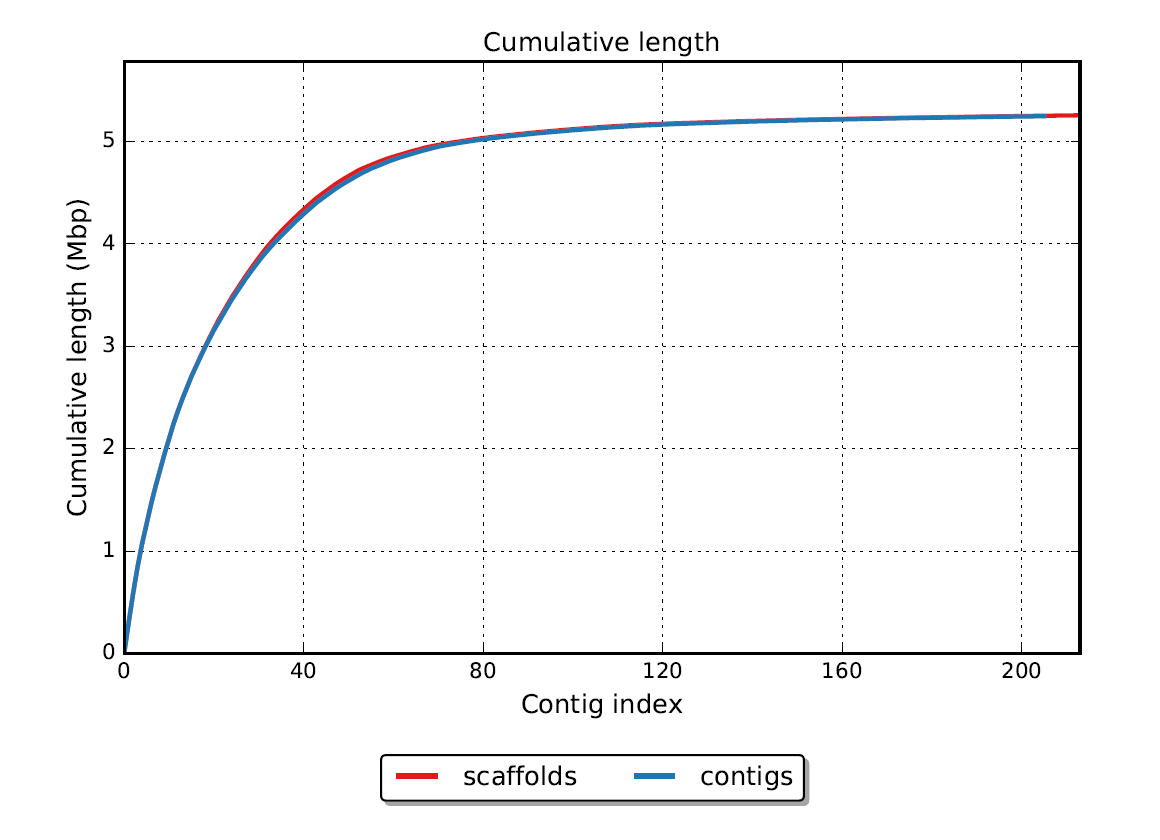
\includegraphics[scale=0.5 ]{images/consca.png} 
\centering \caption{Assessment of the quality of the paired processed data after using SPAdes}
\label{scacof}
\end{figure}
The information related to the quality of the resulting assembly after SPAdes usage is available in lab journal. 




\section{Discussion}

 
%\newpage 
%\newpage 
\begin{thebibliography}{9}
 \bibitem{data}
 Datasets:  (forward and reverse) \\
SRR292678: \\
https://d28rh4a8wq0iu5.cloudfront.net/bioinfo/SRR292678sub\_S1\_L001\_R1\_001.fastq.gz \\ https://d28rh4a8wq0iu5.cloudfront.net/bioinfo/SRR292678sub\_S1\_L001\_R2\_001.fastq.gz \\
SRR292862: \\
https://d28rh4a8wq0iu5.cloudfront.net/bioinfo/SRR292862\_S2\_L001\_R1\_001.fastq.gz \\ https://d28rh4a8wq0iu5.cloudfront.net/bioinfo/SRR292862\_S2\_L001\_R2\_001.fastq.gz \\
SRR292770: \\
https://d28rh4a8wq0iu5.cloudfront.net/bioinfo/SRR292770\_S1\_L001\_R1\_001.fastq.gz \\
https://d28rh4a8wq0iu5.cloudfront.net/bioinfo/SRR292770\_S1\_L001\_R2\_001.fastq.gz

 \bibitem{fc}
 Fastqc : https://www.bioinformatics.babraham.ac.uk/projects/fastqc/
 
 
 \bibitem{jellyfish}
 Guillaume Marcais and Carl Kingsford, A fast, lock-free approach for efficient parallel counting of occurrences of k-mers. Bioinformatics (2011) 27(6): 764-770 (first published online January 7, 2011) doi:10.1093/bioinformatics/btr011
 
 
 \bibitem{spades}
SPAdes: http://cab.spbu.ru/software/spades/


\bibitem{quost}
QUAST: http://quast.bioinf.spbau.ru/

\end{thebibliography}




\end{document}
